\documentclass[12pt,a4paper]{report}

% Packages
\usepackage{geometry}
\geometry{margin=1in}
\usepackage{graphicx}
\usepackage{setspace}
\usepackage{hyperref}
\usepackage{tocloft}
\usepackage{longtable}
\usepackage{listings}
\usepackage{xcolor}

\lstset{
basicstyle=\ttfamily\small,
breaklines=true,
frame=single
}

\begin{document}

%------------------------------------------------
% TITLE PAGE
%------------------------------------------------

\begin{titlepage}
    \centering
    \vspace*{2cm}
    
    {\Huge \textbf{Call Graph and Coupling}}\\[0.5cm]
    {\Large \textbf{NexusNotes}}\\[0.5cm]
    {\large Centralized Academic Resource Platform}\\[2cm]
    
    \textbf{Project Team: Code Club}\\[0.5cm]
    Ramasani Adi Pranav -- 24CSB0A57\\
    Syed Mohammad Sami -- 24CSB0A77\\
    Janapala Harsha Vardhan Reddy -- 24CSB0A28\\[2cm]
    
    \vfill
    {\large \textbf{Version 1.0}}\\
    {\large \today}
    
\end{titlepage}

\tableofcontents
\newpage

%------------------------------------------------
% INTRODUCTION
%------------------------------------------------

\chapter{Introduction}

NexusNotes is a centralized academic resource management platform designed to organize and distribute academic materials efficiently. The system allows students to upload, search, and download academic resources while administrators monitor and manage the platform. 

The system architecture consists of several modules including authentication, resource management, search and retrieval, and administration. These modules interact to ensure secure access, structured resource storage, and efficient information retrieval.

This document presents the source code structure, call graphs, module structure, and coupling relationships of the NexusNotes platform.

%------------------------------------------------
% SOURCE CODE
%------------------------------------------------

\chapter{Source Code}

\section{Student Controller}

\begin{lstlisting}
exports.uploadAcademicResource = async (req, res) => {
 const { title, subject, category, tags } = req.body;
 const file = req.file;

 if (!validateFile(file)) {
  return res.status(400).json({ error: 'Invalid file' });
 }

 const resource = await saveResource(
  req.user.id,
  title,
  subject,
  category,
  tags,
  file.path
 );

 res.status(201).json({ success: true, resource });
};

function validateFile(file){
 return file.size <= 50*1024*1024;
}

async function saveResource(){
 // store resource
}
\end{lstlisting}
\newpage
\section{Admin Controller}

\begin{lstlisting}
exports.manageUserRoles = async (req,res)=>{

 const {targetUserId,newRole} = req.body;

 if(!verifyAdminPrivileges(req.user)){
  return res.status(403).json({error:"Unauthorized"});
 }

 const updatedUser =
  await updateUserRole(targetUserId,newRole);

 res.status(200).json({success:true,updatedUser});
}

function verifyAdminPrivileges(user){
 return user.role === 'Administrator';
}
\end{lstlisting}

\section{Authentication Controller}

\begin{lstlisting}
exports.login = async(req,res)=>{

 const {email,password} = req.body;

 const user = await checkCredentials(email,password);

 if(user){
  const token = generateToken(user._id,user.role);
  res.status(200).json({token});
 }
}

function generateToken(id,role){
 return jwt.sign({id,role},"SECRET",{expiresIn:"1d"});
}
\end{lstlisting}

%------------------------------------------------
% CALL GRAPH
%------------------------------------------------

\chapter{Call Graph Diagrams}

Call graphs illustrate how functions within the system interact with each other during execution.

\section{Student Module Call Graph}

\begin{figure}[h]
\centering
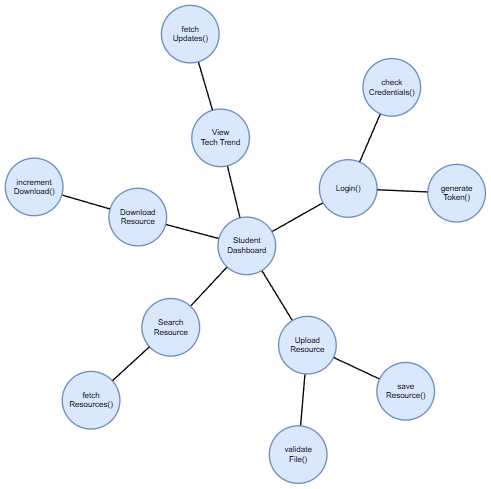
\includegraphics[width=0.8\textwidth]{graphviz(1).png}
\caption{Student Module Call Graph}
\end{figure}

\section{Student Module Call Graph}

\textbf{1. Student Dashboard as the Primary Controller}

\begin{itemize}
\item The Student Dashboard acts as the central interface through which students interact with the NexusNotes platform.
\item It connects all major functionalities such as uploading resources, searching materials, downloading files, and viewing technology updates.
\item This centralized structure simplifies user interaction and ensures organized navigation within the system.
\end{itemize}

\textbf{2. Authentication and Login Process}

\begin{itemize}
\item The Login() function initiates the authentication process for the student.
\item The system calls checkCredentials() to verify whether the entered email and password match the stored user data.
\item Once verification is successful, generateToken() creates an authentication token that allows secure access to system features.
\item This process ensures that only authorized students can upload or access academic resources.
\end{itemize}

\textbf{3. Resource Upload Process}

\begin{itemize}
\item Upload Resource is responsible for allowing students to contribute academic materials such as lecture notes, project reports, or presentations.
\item The validateFile() function checks whether the uploaded file meets system requirements such as supported formats and size limits.
\item Once validated, saveResource() stores the resource in the database along with its metadata including title, subject, category, and tags.
\item This ensures that uploaded resources are properly stored and categorized within the repository.
\end{itemize}

\textbf{4. Resource Search and Retrieval}

\begin{itemize}
\item Search Resource allows students to locate academic materials using keywords or filters.
\item The system calls fetchResources() to retrieve relevant materials from the database.
\item The retrieved resources are displayed to the student based on relevance and availability.
\item This functionality ensures quick access to study materials stored in the system.
\end{itemize}

\textbf{5. Resource Download Process}

\begin{itemize}
\item Download Resource enables students to obtain academic files for offline study.
\item The incrementDownload() function updates the download count of the resource.
\item Tracking download statistics helps the system identify popular and frequently accessed resources.
\end{itemize}

\textbf{6. Technology Trend Feed}

\begin{itemize}
\item View Tech Trend allows students to stay updated with current developments in technology related to their academic domain.
\item The fetchUpdates() function retrieves curated technology news and updates from external APIs or services.
\item This feature bridges the gap between academic learning and industry trends.
\end{itemize}

\section{Admin Module Call Graph}

\begin{figure}[h]
\centering
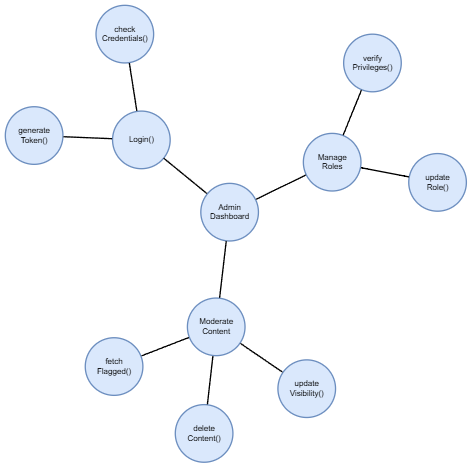
\includegraphics[width=0.8\textwidth]{graphviz.png}
\caption{Admin Module Call Graph}
\end{figure}
\newpage

\textbf{1. Admin Dashboard as the Central Control Unit}

\begin{itemize}
\item The Admin Dashboard serves as the main control interface for administrative activities.
\item It connects administrative tasks such as role management, content moderation, and system monitoring.
\item This centralized structure enables administrators to efficiently manage the platform.
\end{itemize}

\textbf{2. Authentication and Security}

\begin{itemize}
\item The Login() function begins the administrator authentication process.
\item The system verifies credentials using checkCredentials().
\item If authentication is successful, generateToken() generates a secure token that grants access to administrative functionalities.
\item This ensures that only authorized administrators can modify system data.
\end{itemize}

\textbf{3. User Role Management}

\begin{itemize}
\item Manage Roles allows administrators to assign or modify roles of system users.
\item verifyPrivileges() ensures that the current user has administrator permissions.
\item updateRole() updates the role information of the selected user in the database.
\item This functionality helps maintain proper access control across the system.
\end{itemize}

\textbf{4. Content Moderation}

\begin{itemize}
\item Moderate Content allows administrators to review resources uploaded by students.
\item fetchFlagged() retrieves content that has been reported or flagged for review.
\item deleteContent() removes inappropriate or invalid resources from the system.
\item updateVisibility() changes the visibility status of resources, allowing administrators to approve or restrict access.
\item This ensures that only verified and relevant academic materials remain available on the platform.
\end{itemize}

%------------------------------------------------
% MODULE STRUCTURE
%------------------------------------------------

\chapter{Module Structure Diagram}

\begin{figure}[h]
\centering
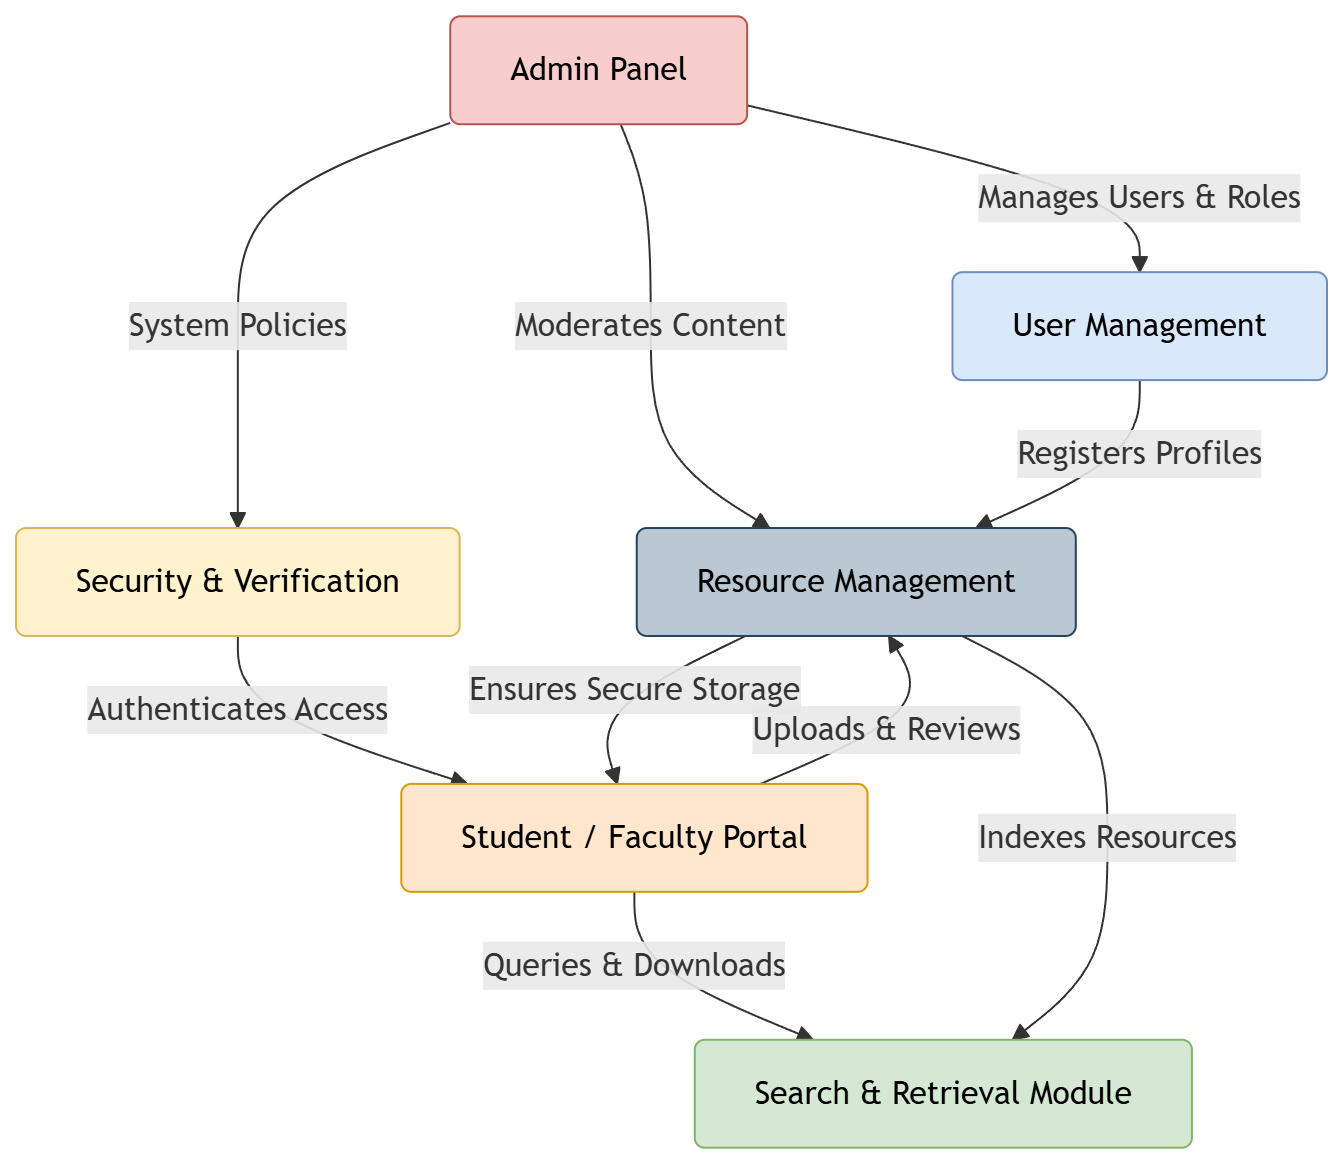
\includegraphics[width=0.9\textwidth]{mermaid-diagram-2026-03-07-151448.png}
\caption{Module Structure of NexusNotes}
\end{figure}
\newpage

\textbf{Explanation}

\textbf{1. Security Module}

\begin{itemize}
\item The Security Module manages authentication and access control for users.
\item Authentication verifies the identity of users before granting system access.
\item Security verification ensures that only authorized individuals can interact with the platform.
\item This module protects the system from unauthorized usage.
\end{itemize}

\textbf{2. Admin Module}

\begin{itemize}
\item The Admin Module manages platform operations and governance.
\item Admin Panel acts as the central interface for administrators.
\item User Management controls user roles and permissions.
\item Content Moderation ensures that uploaded resources meet academic standards.
\end{itemize}

\textbf{3. Resource Module}

\begin{itemize}
\item The Resource Module handles all operations related to academic materials.
\item Upload Resource allows users to contribute academic files.
\item Download Resource enables students to retrieve study materials.
\item Resource Operations organize and manage stored academic content.
\end{itemize}

\textbf{4. Search and Retrieval Module}

\begin{itemize}
\item The Search Engine processes user queries.
\item Query Processing interprets search keywords and filters.
\item Content Indexing organizes stored resources to enable fast retrieval.
\item This module ensures efficient searching of academic materials.
\end{itemize}

%------------------------------------------------
% COUPLING DIAGRAM
%------------------------------------------------

\chapter{Coupling and Cohesion Analysis}

\begin{figure}[h]
\centering
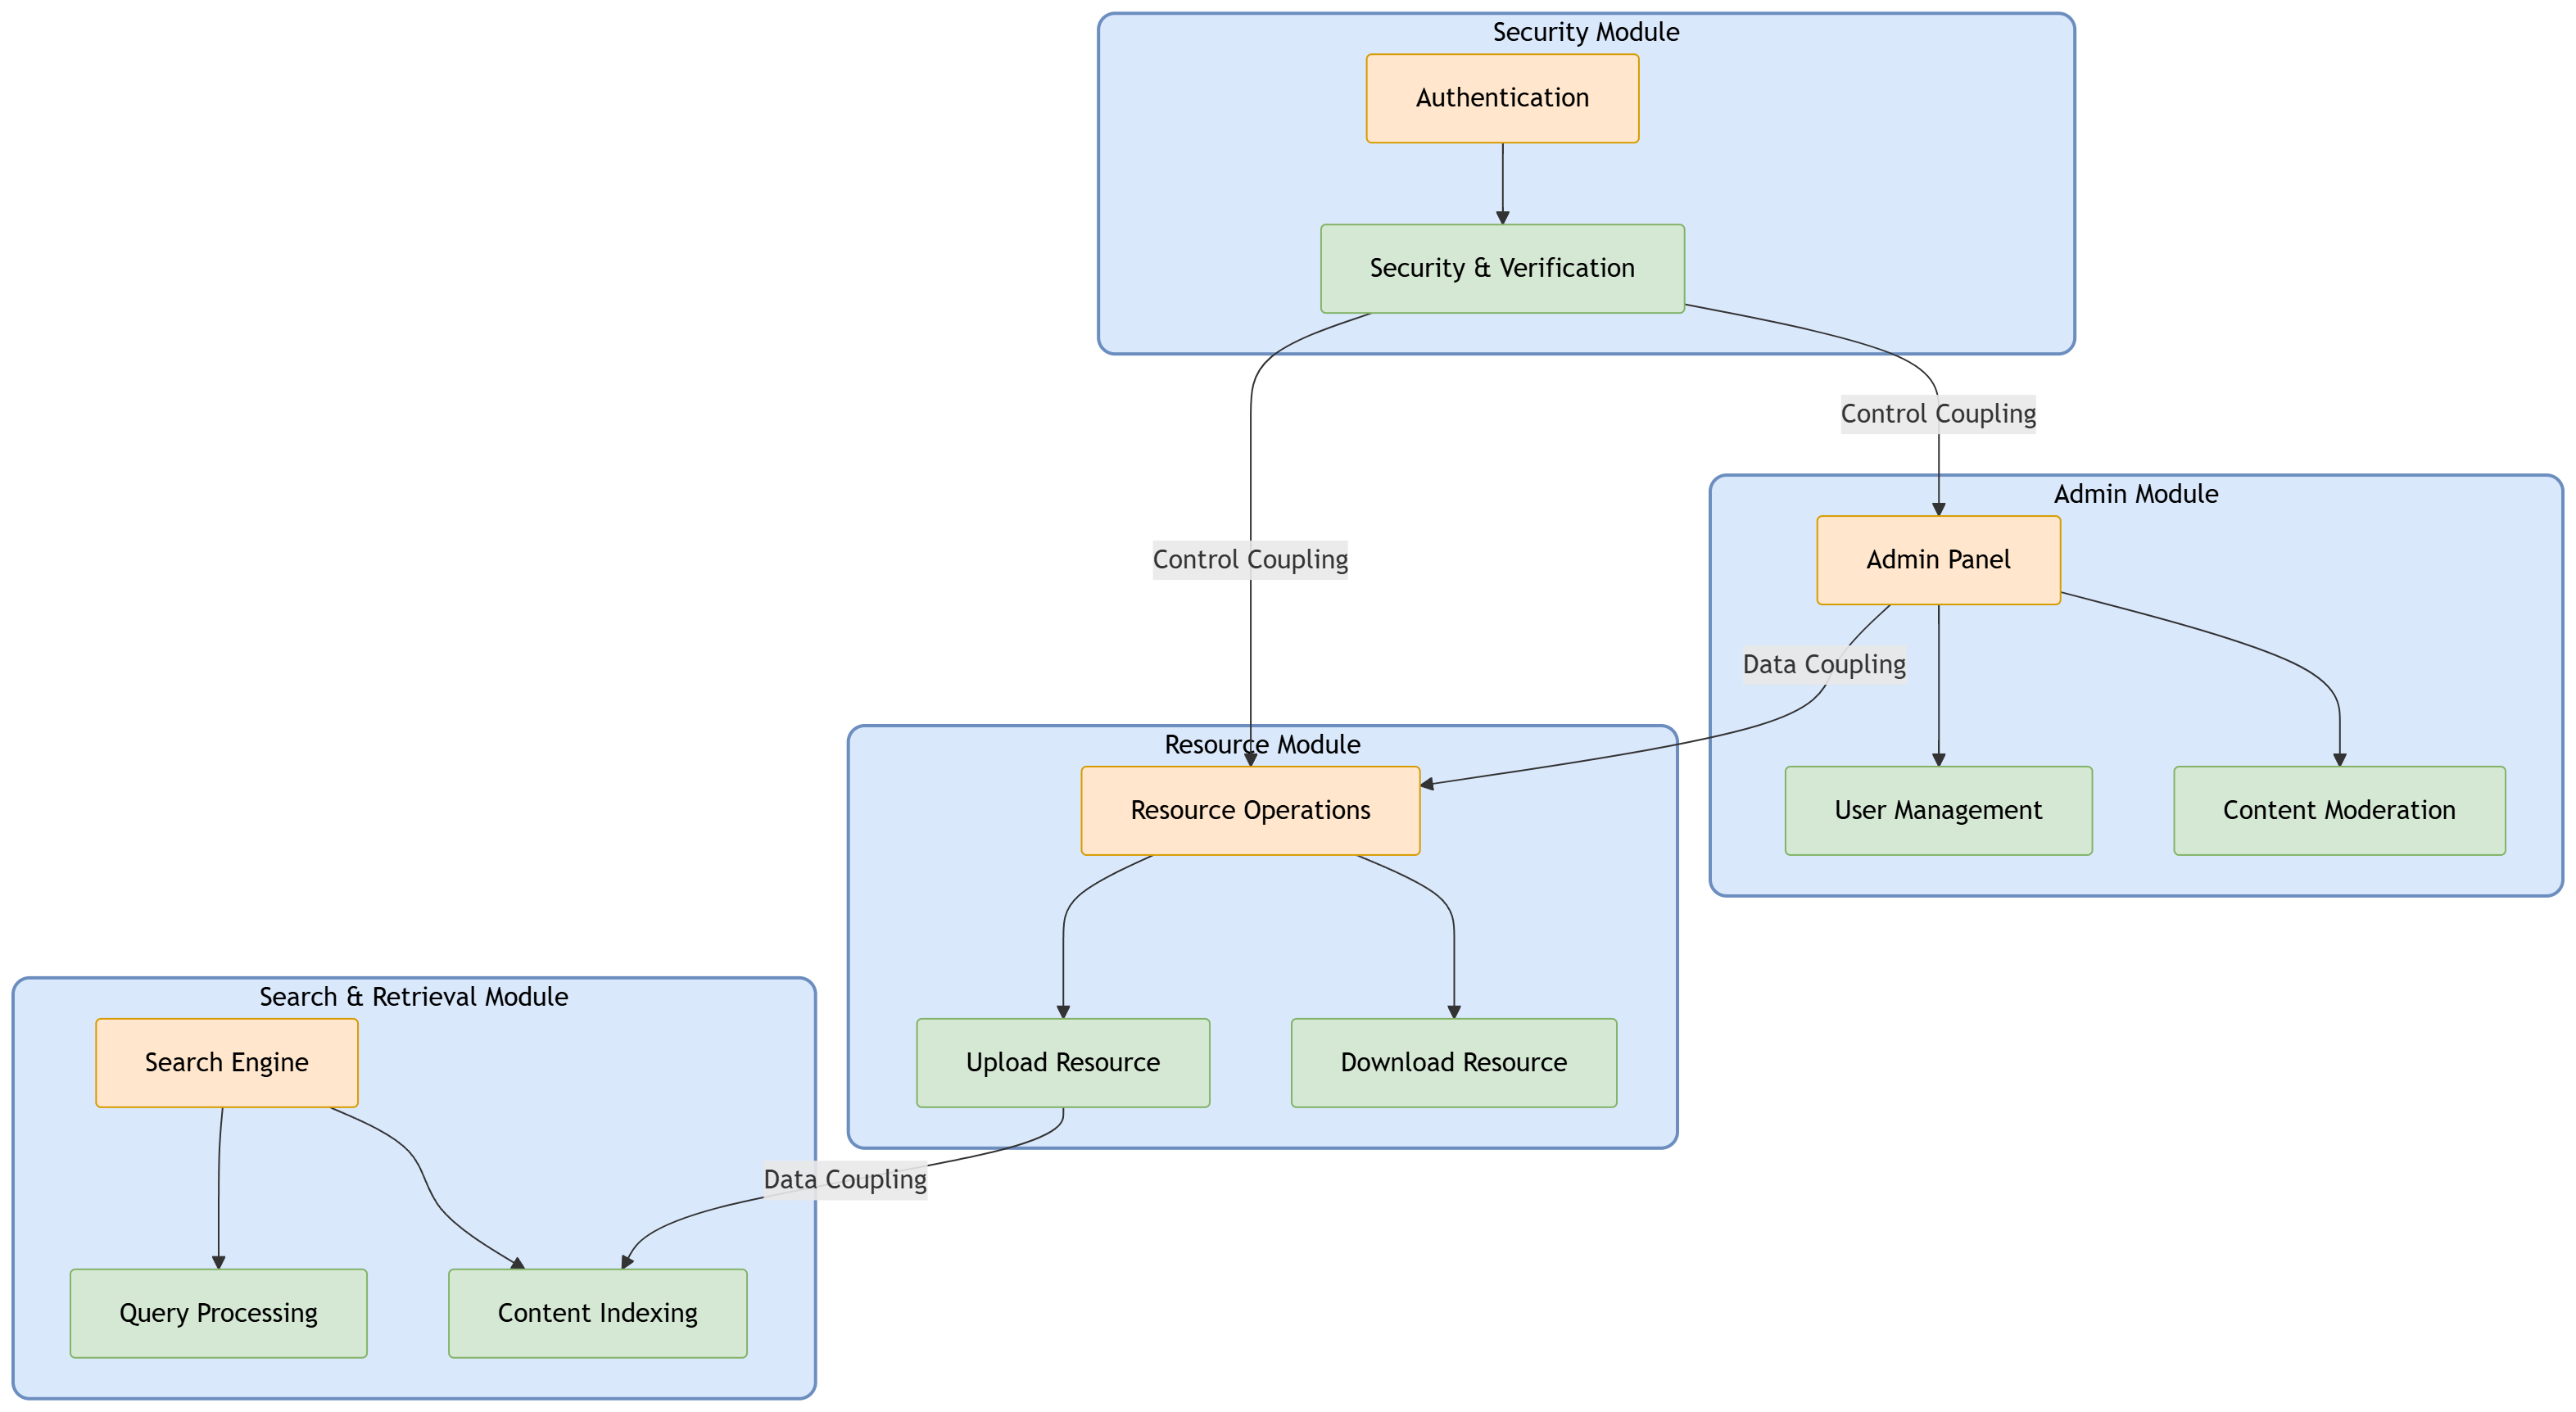
\includegraphics[width=0.9\textwidth]{mermaid-diagram-2026-03-07-151721.png}
\caption{System Coupling Diagram}
\end{figure}

\section{Cohesion}

Cohesion refers to the degree to which the elements within a module belong together.

\begin{itemize}
\item Each module in NexusNotes performs a specific and well-defined function.
\item Security Module focuses only on authentication and verification.
\item Admin Module manages system governance and user roles.
\item Resource Module handles uploading, downloading, and storage of academic materials.
\item Search Module manages searching and indexing operations.
\end{itemize}

\textbf{Benefits of High Cohesion}

\begin{itemize}
\item Improves maintainability of the system.
\item Allows independent modification of modules.
\item Enhances code readability and debugging efficiency.
\end{itemize}

\section{Coupling}

Coupling refers to the level of dependency between different modules.

\textbf{Control Coupling}

\begin{itemize}
\item Security Module → Admin Module  
Authentication controls access to administrative functionalities.
\item Security Module → Resource Module  
User verification determines whether a user can upload or download resources.
\end{itemize}

\textbf{Data Coupling}

\begin{itemize}
\item Resource Module → Search Module  
Uploaded resources are indexed for search operations.
\item Admin Module → Resource Module  
Administrative moderation actions update resource visibility and availability.
\end{itemize}

\textbf{Impact of Coupling}

\begin{itemize}
\item Controlled module interaction maintains system integrity.
\item Data coupling ensures efficient information exchange between modules.
\item Balanced coupling improves modularity while preserving functionality.
\end{itemize}

%------------------------------------------------

\chapter{Conclusion}

The NexusNotes system demonstrates a modular architecture with clear separation of responsibilities across different components. The call graph diagrams illustrate how system functions interact, while the module structure diagram shows the overall organization of the platform.

Through effective cohesion and controlled coupling between modules, the system ensures maintainability, scalability, and secure management of academic resources.

\end{document}